    %%%%%%%%%%%%%%%%%%%%%%%%%%%%%%%%%%%%%%%%%%%%%%%%%%%%%%%%%%%%%%%%%%%%%%%%%%%%%%%%
%2345678901234567890123456789012345678901234567890123456789012345678901234567890
%        1         2         3         4         5         6         7         8


\documentclass[letterpaper, 10 pt, conference]{ieeeconf}  % Comment this line out
                                                          % if you need a4paper
%\documentclass[a4paper, 10pt, conference]{ieeeconf}      % Use this line for a4
                                                          % paper

\IEEEoverridecommandlockouts                              % This command is only
                                                          % needed if you want to
                                                          % use the \thanks command
\overrideIEEEmargins
% See the \addtolength command later in the file to balance the column lengths
% on the last page of the document
\usepackage[utf8]{inputenc}
\usepackage[brazil]{babel}
\usepackage{minted}
\usepackage{graphicx,url}
\usepackage[gray]{xcolor}


% The following packages can be found on http:\\www.ctan.org
%\usepackage{graphics} % for pdf, bitmapped graphics files
%\usepackage{epsfig} % for postscript graphics files
%\usepackage{mathptmx} % assumes new font selection scheme installed
%\usepackage{times} % assumes new font selection scheme installed
%\usepackage{amsmath} % assumes amsmath package installed
%\usepackage{amssymb}  % assumes amsmath package installed

\title{\bf INF01008 - Programação distribuída e paralela\\ Análise de message brokers}

\author{ \parbox{3 in}{\centering Lucas Augusto Tansini
        \\
        Instituto de Informática\\
        Universidade Federal do Rio Grande do Sul\\
        Porto Alegre, Brasil\\
        {\tt\small lucas.tansini@inf.ufrgs.br}}
        \hspace*{ 0.5 in}
        \parbox{3 in}{ \centering Lucas Valandro da Rocha\\
        Instituto de Informática \\
        Universidade Federal do Rio Grande do Sul\\
        Porto Alegre, Brasil\\
        {\tt\small lvrocha@inf.ufrgs.br}}
}


\begin{document}



\maketitle
\thispagestyle{empty}
\pagestyle{empty}


%%%%%%%%%%%%%%%%%%%%%%%%%%%%%%%%%%%%%%%%%%%%%%%%%%%%%%%%%%%%%%%%%%%%%%%%%%%%%%%%
\begin{abstract}

Este trabalho tem como objetivo avaliar e comparar o desempenho de Message Brokers (sistemas
de entrada de dados utilizados para aplicações Big Data e IoT), de forma a variar parâmetros como: número de mensagens e número de filas, por exemplo. O restante deste trabalho se extende em introdução, configuração dos ambientes dos sistemas, variações utilizadas, resultados obtidos e conclusões.

\end{abstract}


%%%%%%%%%%%%%%%%%%%%%%%%%%%%%%%%%%%%%%%%%%%%%%%%%%%%%%%%%%%%%%%%%%%%%%%%%%%%%%%%
\section{INTRODUÇÃO}

Com o aumento do número de dados em diversas aplicações, vê-se necessário a busca de mecanismos para atender demandas altíssimas de comunicação, troca de mensagens e processamento. Dados mostram que, em 2019, aplicações famosas como o Netflix e o Twitter podem gerar até 700 mil horas e 88 mil Tweets em 60 segundos, respectivamente. Com o intuito de suportar a imensa quantidade de dados, módulos intermediários como os \textit{Message Brokers} têm o propósito de auxiliar na troca de mensagens entre aplicações. Os módulos podem desacoplar fortemente as mensagens de suas aplicações, provendo uma facilidade de reuso. Por serem módulos intermediários e desacoplados, os \textit{Message Brokers} provêm aumento de performance, através de comunicação assíncrona. Após um produtor publicar uma mensagem no \textit{broker}, ele pode continuar sua execução tendo a certeza que o consumidor irá receber a mensagem, e também existem maneiras de comunicar o produtor de que o consumidor recebeu a mensagem.  

\section{ATIVIDADES EXECUTADAS}

Para a realização desse trabalho, realizaram-se as seguintes atividades:

\begin{itemize}
\item Modelagem dos dados que ficaram salvos no banco \textit{MongoDB}.
\item Criação dos 5 \textit{datasets} e salvamento dos dados no banco.
\item Configuração dos ambientes em Docker para criação das instâncias do \textit{RabbitMQ e Apache Kafka.}
\item Estudo do funcionamento dos \textit{frameworks} propostos.
\item Desenvolvimento de 2 aplicações em Java para conexão com cada uma instância dos \textit{brokers}, cada aplicação contendo duas configurações, com 1 ou 2 filas.
\item Execução de 10 vezes para cada combinação de \textit{dataset} mais quantidade de filas, totalizando 100 execuções do experimento.
\item Análise dos resultados.
\end{itemize}


\section{CASOS DE ESTUDO}

Para o estudo do funcionamento e desempenho de  \textit{Message Brokers}, foram escolhidos dois \textit{frameworks}: \textit{Apache Kafka}~\cite{c1} e \textit{RabbitMQ}~\cite{c2}. A escolha desses \textit{frameworks} se deu pela facilidade de entendimento, utilização e também pelo grande uso comercial, por empresas como Netflix, Uber, Airbnb, Cisco e LinkedIn.

\subsection{Critérios de avaliação de desempenho}

Para avaliar o desempenho de ambas plataformas, 5 conjuntos de dados com 100, 500, 5.000, 50.000 e 100.000 mensagens foram utilizadas, assim como duas diferentes configurações, utilizando uma ou duas filas, totalizando assim 10 experimentos diferentes para cada plataforma. 

\subsection{Ambiente de teste}

Para realização dos testes de \textit{benchmark} utilizou-se a seguinte configuração:

\begin{itemize}
\item \textit {Rabbit MQ e Kafka} executando dentro de containers Docker.
\item Aplicação escrita em Java executando sobre um processador Intel(R) Core(TM) i5 - 5350U CPU @ 1.8 GHz (2 cores, 4 threads).
\item Banco de dados \textit{MongoDB}, na nuvem, contendo os dados que o produtor envia ao consumidor.
\end{itemize}

\subsection{Estrutura da mensagem}

Os dados que o produtor consome do banco de dados não relacional, o \textit{MongoDB}, correspondem a um cliente genérico, tendo o formato JSON. O tamanho médio de cada registro é de 150 \textit{bytes}.

\begin{figure}[thpb]
      \begin{minted}{json}
{
    "id":1,
    "first_name":"Bobette",
    "last_name":"Habard",
    "email":"bhabard0@t-online.de",
    "gender":"Female",
    "ip_address":"149.7.170.207"
}
      \end{minted}
      \caption{Conteúdo de um registro dos dados lidos pela aplicação.}
      \label{fig:document}
\end{figure}

\section{RABBIT MQ}

O \textit{Rabbit MQ} é a ferramenta \textit{open-source} mais utilizada como \textit{message broker} atualmente, segundo a Pivotal \cite{c2}. Todos os protocolos implementados pelo \textit{Rabbit MQ} permitem que a aplicação produtora consiga confirmar se a mensagem enviada foi recebida pelo \textit{broker}. As aplicações produtoras podem tanto manter uma conexão com o \textit{Rabbit MQ} durante todo seu tempo de execução, ou de maneira mais otimizada, apenas estabelecer essa conexão quando for necessário enviar uma mensagem ao \textit{broker}.

\subsection{Fluxo dos dados}

Quando uma mensagem mensagem será publicada em um \textit{broker}, primeiramente, ela deve passar por uma estrutura chamada \textit{Exchange}. Essa estrutura serve para direcionar corretamente até o \textit{broker}, as mensagens enviadas pela aplicação produtora, podendo ainda ter seu funcionamento alterado através de um parâmetro chamado \textit{exchange type}. Esse parâmetro faz com que essa mensagem seja direcionada para um \textit{broker} específico, ou até para todos disponíveis.


\begin{figure}[ht]
\centering
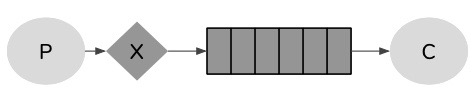
\includegraphics[width=.4\textwidth]{exchange.jpeg}
\caption{Configuração com produtor (P), \textit{exchange} (X), \textit{broker} e consumidor (C).}
\label{fig:exchange}
\end{figure}


\section{APACHE KAFKA}

O \textit{Apache Kafka} é uma plataforma distríbuida de \textit{streaming}. Isso significa, segundo o site oficial \cite{c1}, que ele possui três grandes capacididades:

\begin{itemize}
\item Publicar e consumir \textit{streams} de dados, similar à fila de mensagens.
\item Salvar esses dados garantindo tolerância a falhas.
\item Processar os dados a partir do momento em que eles chegam até o Kafka.
\end{itemize}


\begin{figure}[ht]
\centering
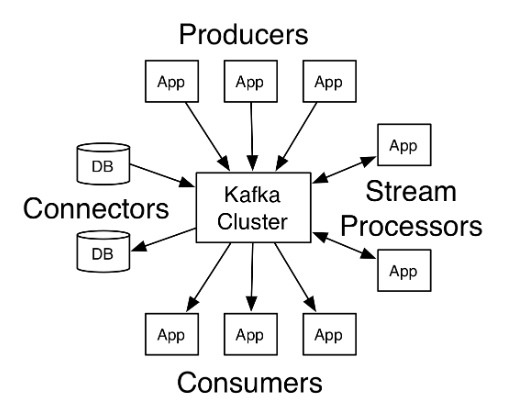
\includegraphics[width=.35\textwidth]{kafka-usage.png}
\caption{Ilustração do funcionamento do Kafka com todas as plataformas que ele pode se comunicar.}
\label{fig:exchange}
\end{figure}

O \textit{Apache Kafka} é recomendado para utilização em dois tipos de aplicações: aplicações de tempo real com fluxo constante de dados, a fim de buscar dados de sistemas e outras aplicações, e também em aplicações de tempo real que transformam fluxos de dados, ou que devem reagir a mudanças em fluxos de dados.

\subsection{Fluxo dos dados}

Os produtores enviam mensagens para o \textit{broker} que separa esse fluxo de dados em estruturas chamadas de \textit{topics}. Cada consumidor inscreve-se em um, ou mais, \textit{topic} a fim de consumir essas mensagens assim que forem publicadas.

\begin{figure}[ht]
\centering
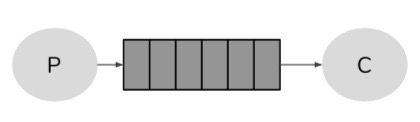
\includegraphics[width=.4\textwidth]{kafka.jpeg}
\caption{Configuração com produtor (P), topic e consumidor (C).}
\label{fig:twoqueues}
\end{figure}

\section{EXPERIMENTO}

\subsection{Configuração I}

A primeira configuração do experimento constinte em um produtor, um \textit{broker} e um consumidor, conforme ilustrado na Fig. 4. Os dados variam de 100 até 100.000, conforme descrito anteriormente, e o tempo medido é entre o produtor publicar todos esses dados no \textit{broker} e o consumidor lê-los completamente.

\begin{figure}[ht]
\centering
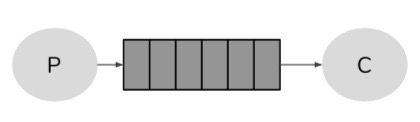
\includegraphics[width=.4\textwidth]{one-queue.jpeg}
\caption{Primeira configuração do experimento, contendo um produtor, um broker e um consumidor.}
\label{fig:onequeue}
\end{figure}

\subsection{Configuração II}

A primeira configuração do experimento decidimos adicionar mais um \textit{broker} e um consumidor, ilustrado pela Fig. 5, a fim de verificarmos o impacto da escalabilidade horizontal dessas estruturas no tempo total medido. Foi feita a mesma variação dos dados de entrada, e o intervalo de tempo medido foi o mesmo. 

\begin{figure}[ht]
\centering
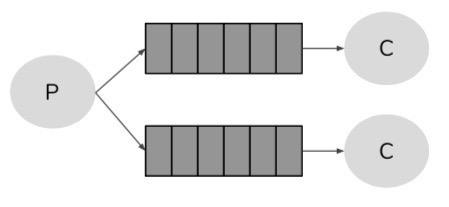
\includegraphics[width=.4\textwidth]{two-queues.jpeg}
\caption{Segunda configuração do experimento, contendo um produtor, dois brokers e dois consumidores.}
\label{fig:twoqueues}
\end{figure}

\section{RESULTADOS}

Conforme apresentado na Fig. ~\ref{grafico_kafka_confg_1}, considerando a média das execuções para a Configuração 1 dos dois \textit{frameworks}, é possível observar que o \textit{Apache Kafka} obteve maior desempenho, chegando ser até 50,1\% mais rápido que o \textit{RabbitMQ}, no maior conjunto de dados. Ainda assim, conforme a Fig. ~\ref{grafico_kafka_confg_2}, é possível observar que na Configuração 2, o \textit{Apache Kafka} continua ganhando em desempenho, obtendo ganhos de até 44,22\%. 

\begin{figure}[!htbp]
\centerline{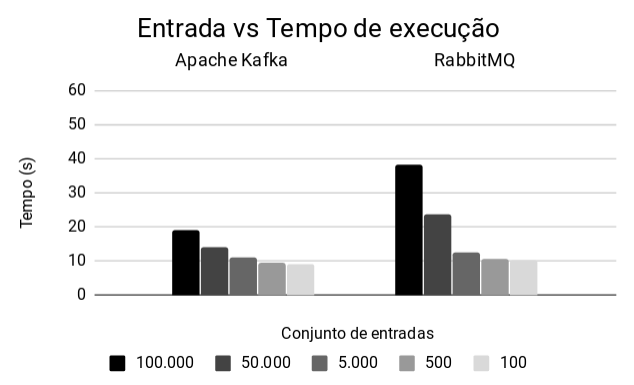
\includegraphics[scale=0.4]{config1KafkavsRabbitMQ.png}}
\caption{Execução do conjunto de dados para a Configuração 1 do \textit{Apache Kafka} (esquerda) vs \textit{RabbitMQ} (direita).}
\label{grafico_kafka_confg_1}
\end{figure}

\begin{figure}[!htbp]
\centerline{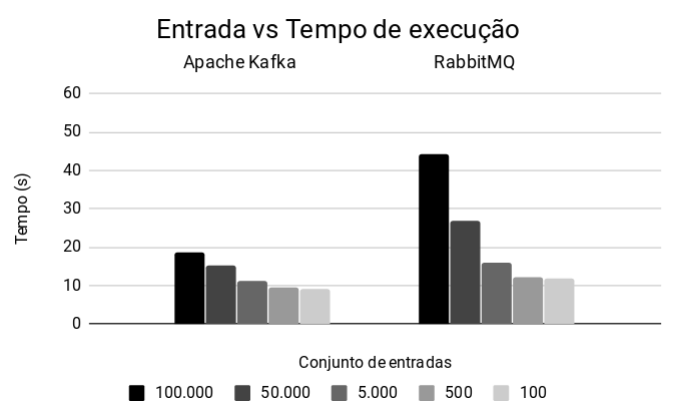
\includegraphics[scale=0.4]{confg2.png}}
\caption{Execução do conjunto de dados para a Configuração 2 do \textit{Apache Kafka} (esquerda) vs \textit{RabbitMQ} (direita).}
\label{grafico_kafka_confg_2}
\end{figure}



\section{CONCLUSÃO}

A utilização de \textit{Message Brokers} em uma aplicação com processamento distríbuido permite que o desenvolvedor realize soluções altamente escaláveis, que lidem com uma enorme quantidade de dados, e também com fluxos constantes de dados, podendo manipulá-los de várias maneiras distintas. \\
Após executar todos os experimentos, concluiu-se que o \textit{Apache Kafka} é mais rápido que o \textit{RabbitMQ} pelas seguintes razões:

\begin{itemize}
\item Não realiza cópia de dados - O \textit{Apache Kafka} realiza chamadas do \textit{kernel} do sistema operacional diretamente. Esse processo é chamado de \textit{Zero-copy}, basicamente ele permite com que a CPU realize outras tarefas enquanto a cópia dos dados é realizada paralelamente em outra parte da máquina \cite{c5}.
\item Organiza os dados em grupos, minimizando a latência realizada em copiar todos os dados e suas dependências para realizar o processamento. 
\item Reduz o acesso randômico em disco, de forma a não realizar muitas operações de \textit{I/O}.
\end{itemize}





\begin{thebibliography}{99}

\bibitem{c1} https://kafka.apache.org/
\bibitem{c2} https://www.rabbitmq.com/
\bibitem{c3} https://en.wikipedia.org/wiki/RabbitMQ
\bibitem{c4} https://en.wikipedia.org/wiki/Message\_broker
\bibitem{c5} https://en.wikipedia.org/wiki/Zero-copy
\end{thebibliography}




\end{document}
